% ****** Start of file apssamp.tex ******
%
%   This file is part of the APS files in the REVTeX 4.2 distribution.
%   Version 4.2a of REVTeX, December 2014
%
%   Copyright (c) 2014 The American Physical Society.
%
%   See the REVTeX 4 README file for restrictions and more information.
%
% TeX'ing this file requires that you have AMS-LaTeX 2.0 installed
% as well as the rest of the prerequisites for REVTeX 4.2
%
% See the REVTeX 4 README file
% It also requires running BibTeX. The commands are as follows:
%
%  1)  latex apssamp.tex
%  2)  bibtex apssamp
%  3)  latex apssamp.tex
%  4)  latex apssamp.tex
%
\documentclass[%
 reprint,
%superscriptaddress,
%groupedaddress,
%unsortedaddress,
%runinaddress,
%frontmatterverbose, 
%preprint,
%preprintnumbers,
%nofootinbib,
%nobibnotes,
%bibnotes,
 amsmath,amssymb,
 aps,
%pra,
%prb,
%rmp,
%prstab,
%prstper,
%floatfix,
]{revtex4-2}

\usepackage{graphicx}% Include figure files
\usepackage{dcolumn}% Align table columns on decimal point
\usepackage{bm}% bold math

\newcommand\abs[1]{\left|#1\right|}
\newcommand\bra[1]{\left| #1 \right \rangle}
\newcommand\ket[1]{\left \langle #1 \right |}

\begin{document}

\preprint{APS/123-QED}

\title{Coulomb interaction driven entanglement with electrons on helium}

% Force line breaks with \\

\date{\today}% It is always \today, today,
             %  but any date may be explicitly specified

%\begin{abstract}
%An article usually includes an abstract, a concise summary of the work
%covered at length in the main body of the article. 
%\begin{description}
%\item[Usage]
%Secondary publications and information retrieval purposes.
%\item[Structure]
%You may use the \texttt{description} environment to structure your abstract;
%use the optional argument of the \verb+\item+ command to give the category of each item. 
%\end{description}
%\end{abstract}

%\keywords{Suggested keywords}%Use showkeys class option if keyword
                              %display desired
\maketitle

%\tableofcontents
\section{Introduction} % Morten + Johannes + Niyaz
Entanglement is the fundamental characteristic that distinguishes
quantum systems composed of two or more coupled objects from their classical counterparts. The study of entanglement in precisely engineered quantum systems with countably many degrees of freedom is at the forefront of modern physics and is a key resource in quantum information science (QIS). This is particularly true in the development of two-qubit logic for quantum computation. Two-qubit entangling gates have been demonstrated in a wide variety of physical systems used in present-day quantum computing, including superconducting circuits~\cite{Steffen1423}, tapped ions~\cite{}, semiconductor quantum dots~\cite{Li809}, color-center defects in diamond~\cite{}, and neutral atoms in optical lattices~\cite{Saffman1010} just to name several. 




Describe problems in these systems.

Electrons on helium is another qubit platform. Here 2 qubit gates have never been discussed in a proper manner.

Coulomb interaction mediated entanglement / Forster interaction

Our work's place in this field

%Electrons on helium represent a promising platform for investigating strongly-coupled qubits. Therefore a systematic investigation of the controlled generation of entanglement between two trapped electrons under the influence of coherent microwave driving pulses, taking into account the effects of the Coulomb interaction between electrons, is of significant importance for quantum information processing using trapped electrons.

\section{Sample, geometry considerations} % Niyaz writes this
%general information about electrons on helium
Surface state electrons (SSE) 'floating' above liquid helium originates from quantization of electron's perpendicular to the surface motion in a trapping potential formed by attractive force from image charge and a large $\sim$ 1 eV barrier at the liquid-vacuum interface. At low temperatures the SSE are trapped in the lowest Rydberg state for vertical motion some 11 nm above the helium surface, which is perfectly clean and has a permittivity close to that of vacuum. The weak interaction with enviorment, which is mainly governed by interaction with quantized surface capillary waves (ripplons) and bulk phonons, ensures long coherence times - a vital ingredient for any qubit platform. SSE's in-plane motion can be further localized by using microdevices on the length scales approaching the interelectron separation (at the order of one micron). 

\begin{figure}
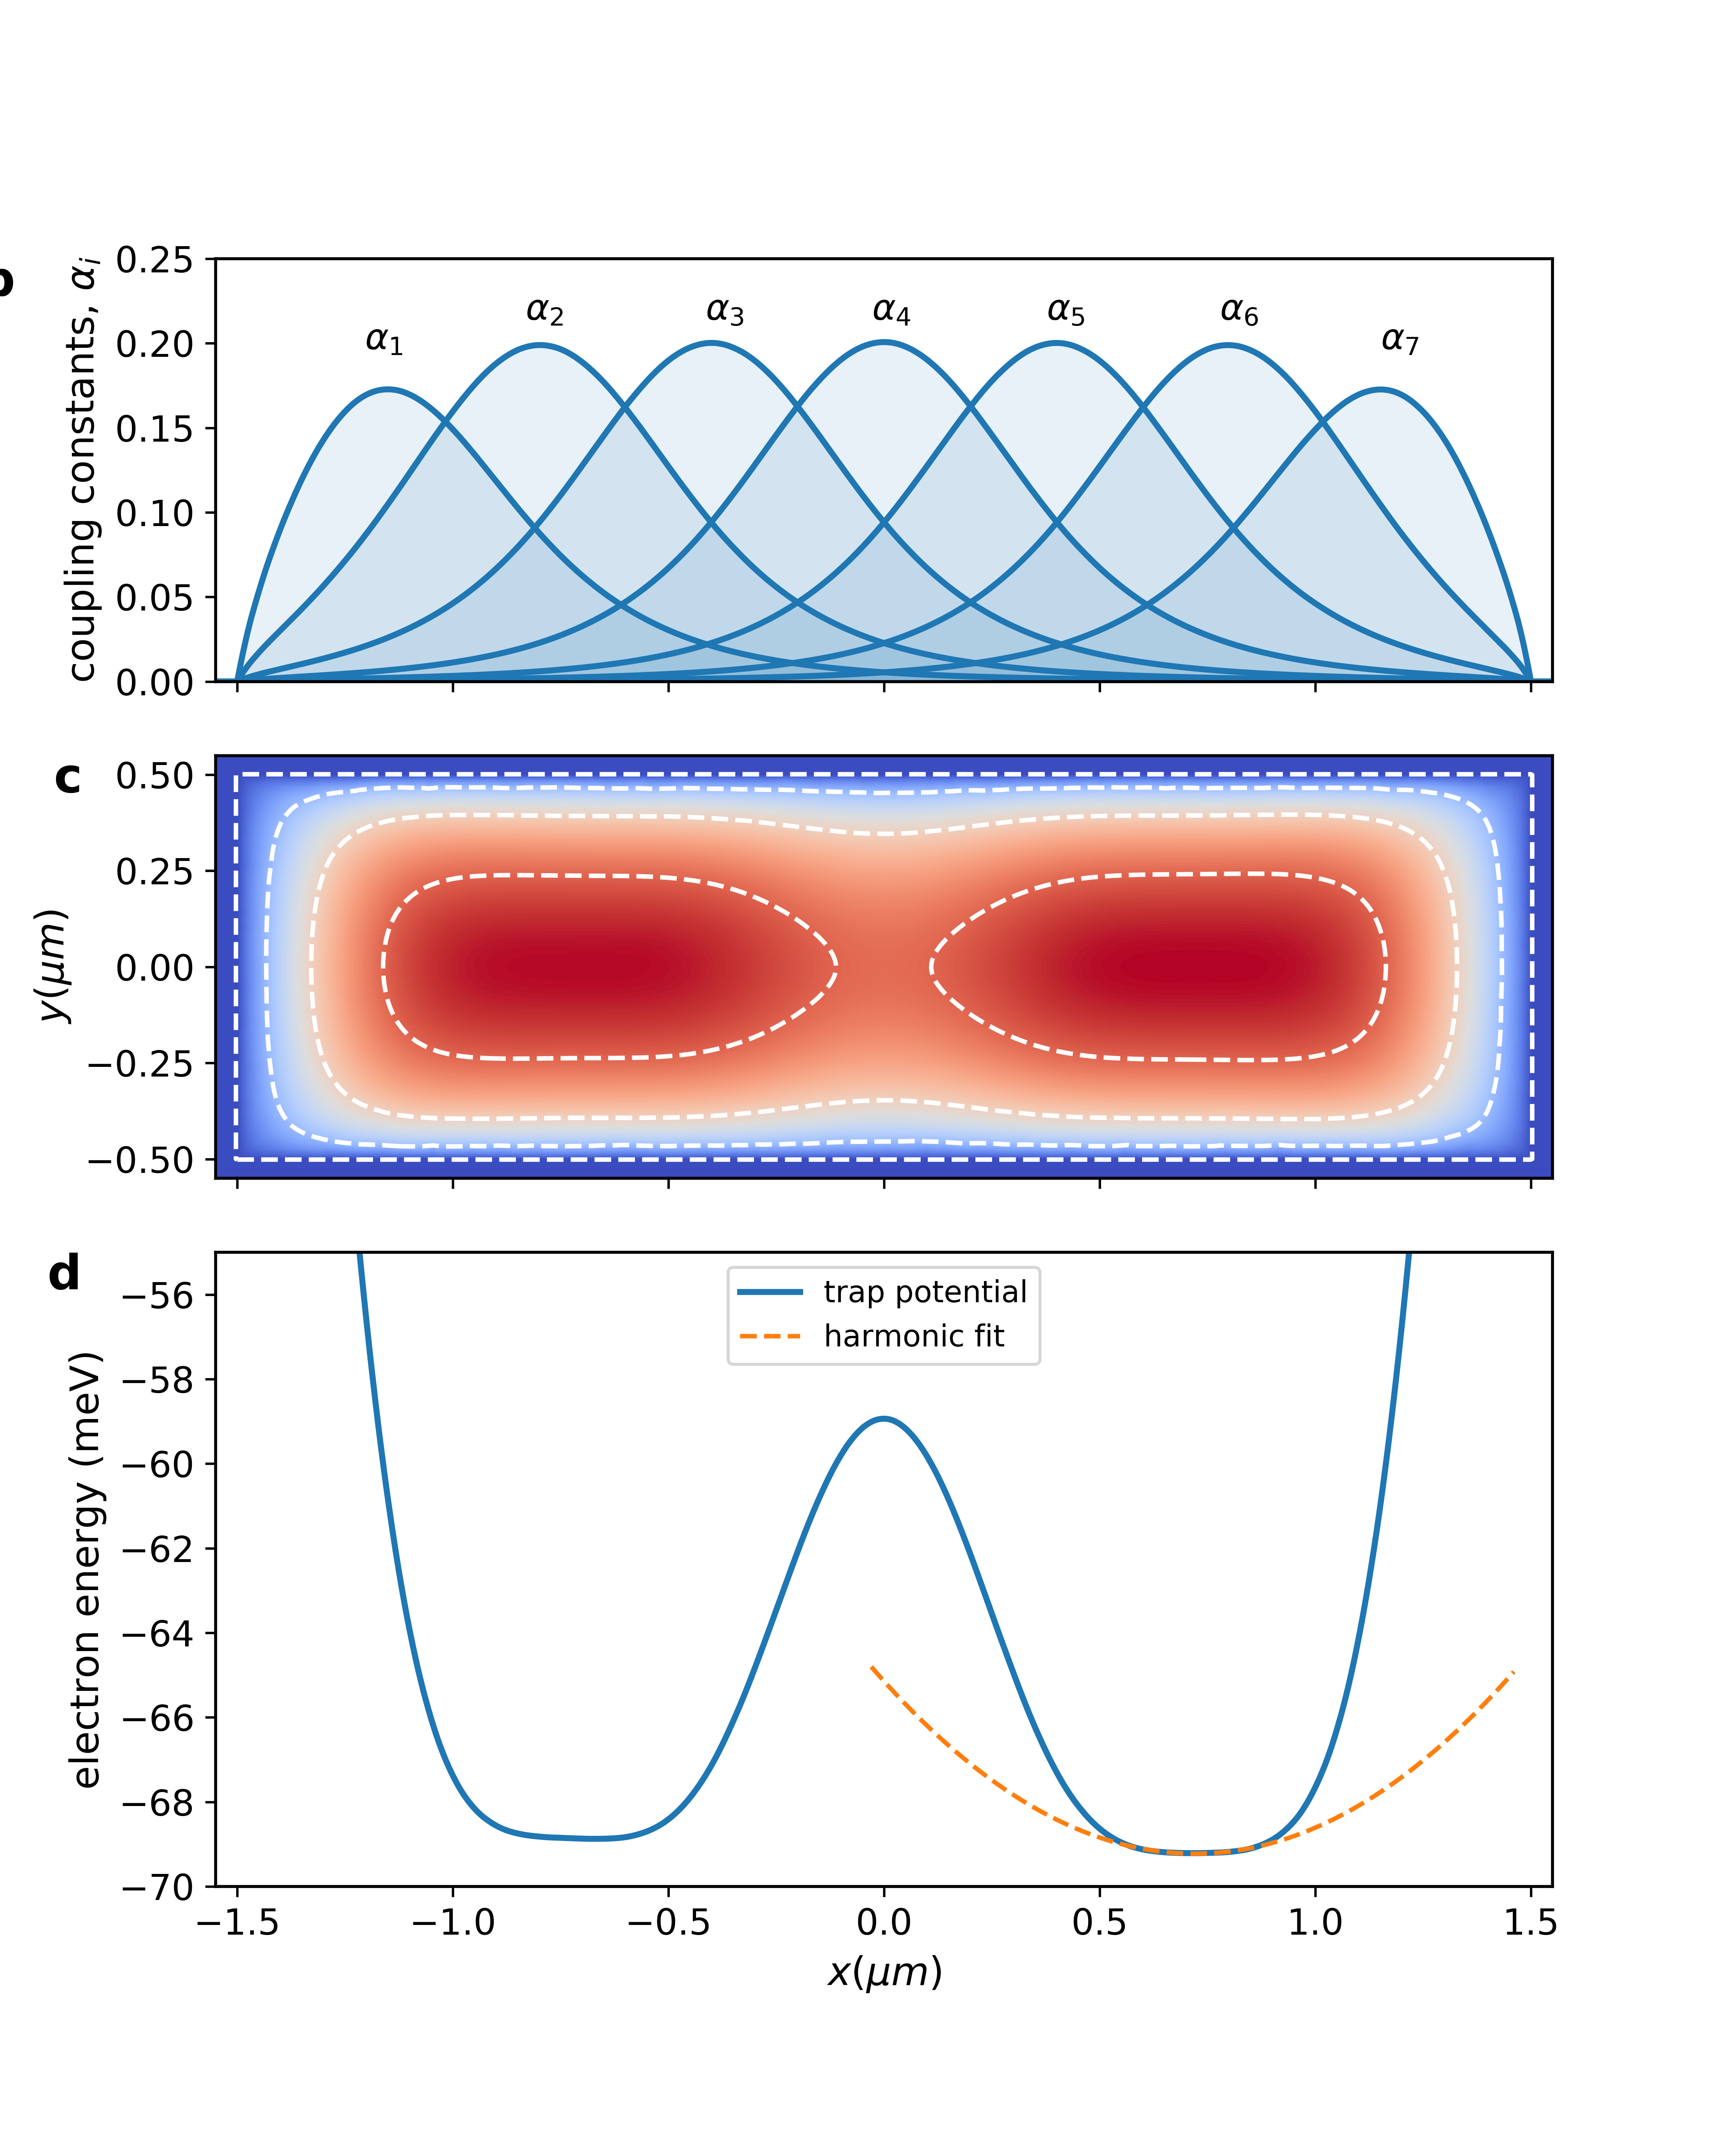
\includegraphics[width=0.49\textwidth]{Fig1.png}
\caption{\label{fig3} (a) Figure caption.}
\end{figure}

\section{Computational Methods} % Hakon, Oyvind

\section{Results and Discussion} % all of us

\section{Conclusions} % we can wait to write this one until the end

\section{\label{sec:level1}Problem: Many-level system interacting with EM field}

We start with the following problem in general form: we have a quantum-mechanical system described with Hamiltonian $H_0$ and states $\bra{n}$ being eigenfunctions of $H_0$: $H_0 \bra{n} = E_n \bra{n}$. we would like to know how these states evolve in time in the presence of time-varying electric field. The interaction of quantum system with electric field is described by Hamiltonian $ H_i = - \mathbf{E}(t) \mathbf{d}$, where $\mathbf{E}(t) = \mathbf{\mathcal{E}}_0 \cos \omega t$ and $\mathbf{d}$ is the dipole moment of the quantum system. Note, here we use dipole approximation (wavelength of the EM filed is much larger than characteristic size of the quantum system wavefunction). The evolution of quantum wavefunction is governed by Schrodinger equation:
\begin{equation}
 i \dot{\psi} = H \psi
\label{eq1}.
\end{equation}
where $H = H_0 + H_i$ (note, $\hbar = 1$). We seek the solution in the form $\psi(t) = \sum_n C_n(t) e^{-i E_n t}$. We plug this solution into Eq.~\ref{eq1} and get the following answer:
\begin{equation}
 i \dot{C_m} = -\frac{1}{2} \mathbf{\mathcal{E}}_0 \sum_{\alpha} \sum_{n} C_n e^{i \omega_{mn} t + i \alpha \omega t} \mathbf{d}_{mn}
\label{eq2},
\end{equation}
\begin{equation}
 \langle m\bra{n} = \delta_{mn}, \ket{m} \mathbf{d} \bra{n} = \mathbf{d}_{mn}, E_m - E_n = \omega_{mn}
\end{equation}
Here we used $\cos \omega t = \frac{1}{2} \sum_{\alpha = \pm} e^{i \alpha \omega t}$. Lets assume the system is in the ground state at $t = 0$, so $C_n(0) = \delta_{n1}$. We integrate Eq.~\ref{eq2} and get an expression:
\begin{equation}
 C_m = \frac{i}{2} \mathbf{\mathcal{E}}_0 \sum_{\alpha} \mathbf{d}_{m1} \frac{e^{i (\omega_{mn} + \alpha \omega) t} - 1}{i (\omega_{m1} + \alpha \omega)} 
\label{eq3}.
\end{equation}
An important condition here is:
\begin{equation}
\abs{\frac{\mathbf{\mathcal{E}}_0 \mathbf{d}_{m1}}{\omega_{m1} \pm \omega}} \ll 1
\label{eq4},
\end{equation}
which defines the 2-level approximation

\begin{acknowledgments}

The work of MHJ is supported by the U.S. Department of Energy, Office of Science, office of Nuclear Physics under grant No. DE-SC0021152 and U.S. National Science Foundation Grants No. PHY-1404159 and PHY-2013047. JP acknowledges support from the National Science Foundation via grant number DMR-2003815 as well as the valuable support of the Cowen Family Endowment at MSU. The work of NRB is supported by a sponsored research grant from EeroQ Corp. JP and NRB thank J.R. Lane and J.M. Kitzman for illuminating discussions.
\end{acknowledgments}
\bibliography{apssamp}% Produces the bibliography via BibTeX.

\end{document}
%
% ****** End of file apssamp.tex ******
